\documentclass[10pt,a4paper]{article}
\usepackage[margin=2.2cm]{geometry}
\usepackage{graphicx}
\usepackage{amsmath,amssymb}
\usepackage[font=small,labelfont=bf]{caption}
\usepackage[hidelinks]{hyperref}
\usepackage{xcolor}
\usepackage{float}
\usepackage[section]{placeins}
\newcommand{\ablFirst}{0.85}
\newcommand{\ablFinal}{0.60}
\newcommand{\redMedOld}{12}
\newcommand{\itsMedOld}{17}
\newcommand{\nMemOld}{478}
\newcommand{\redMedNew}{85}
\newcommand{\itsMedNew}{24}
\newcommand{\nMemNew}{478}
\newcommand{\redBelowFiveOld}{20}
\newcommand{\redBelowFiveNew}{0}
\newcommand{\thkBetter}{94}
\newcommand{\thkN}{96}
\newcommand{\thkMedOld}{14.5}
\newcommand{\thkMedNew}{12.7}
\newcommand{\sOneBetter}{12}
\newcommand{\sOneN}{14}
\newcommand{\sOneOld}{0.85}
\newcommand{\sOneNew}{0.60}
\newcommand{\sOneWorse}{EXP05}
\newcommand{\gwShiftMed}{0.09}
\newcommand{\gwShiftMax}{26.56}
\newcommand{\elaShiftMed}{24}
\newcommand{\uncOld}{2.27}
\newcommand{\uncNew}{2.02}
\newcommand{\nPairs}{96}
\newcommand{\realGwShiftMed}{0.08}

\setlength{\parskip}{3pt}
\renewcommand{\topfraction}{0.9}\renewcommand{\bottomfraction}{0.8}\renewcommand{\textfraction}{0.07}\renewcommand{\floatpagefraction}{0.8}
\newcommand{\mie}{m\,i.e.\,yr$^{-1}$}
\graphicspath{{figures_smb/}}

\title{\textbf{Reworked SMB inference phase}\\[2pt]\large ContinuIX, GROUP\_UNIL method01}
\author{Kejdi Lleshi}
\date{\small Working document, 20 October 2026}

\begin{document}
\maketitle

\noindent The first run of the SMB inference stopped after 10--20 L-BFGS iterations and reduced the loss by a few percent.
We reran \emph{only} the SMB phase of all \nPairs\ experiment--glacier pairs on the saved data-assimilation (DA) results. The DA, the emulator,
the SMB profile ($\Delta z=200$\,m), its regularisation (0.05) and the stopping tolerances are unchanged. The design was tuned on
the synthetic glacier S01, where the true SMB is known, and then applied to everything.

\section*{What changed}
\begin{enumerate}\setlength\itemsep{0pt}
\item \textbf{Domain border.} The 5-cell ramp towards zero thickness at the domain edge now acts only outside the ice mask. Before, it removed
ice from inside the glacier at every step (every glacier except G01 touches the edge).
\item \textbf{Fixed time step.} One step, from the CFL condition of the initial state, ending exactly at $t_2$. Before, the step followed the
speed and overshot $t_2$, so the loss jumped by $\sim$0.05\,m under tiny changes and the line search failed.
\item \textbf{Cheaper line search.} Trial steps run the forward model only; value and slope at the current point are reused.
\item \textbf{Band misfit.} The loss is the RMS of the mean thickness residual in each 50\,m elevation band (before: per-cell RMSE). An
SMB profile can only change band totals, not the redistribution of ice inside a band, which comes from the DA thickness.
\item \textbf{Geodetic term.} The glacier-wide mean SMB is tied to the observed mean thickness change (weight 100).
\end{enumerate}

\begin{figure}[H]
\centering
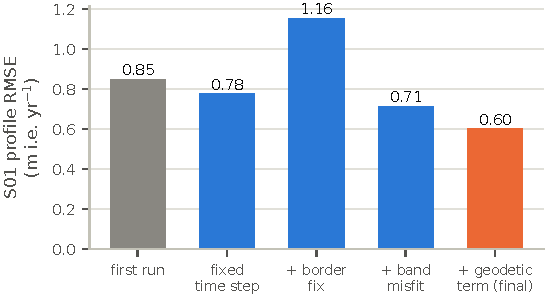
\includegraphics[width=0.58\textwidth]{fig_ablation.pdf}
\caption{S01 (EXP01): family-mean profile error against the prescribed law, adding the changes one by one. The border fix alone worsens S01,
because the old ramp happened to remove over-thick DA ice at the glacier head; the band misfit and the geodetic term give the improvement.}
\end{figure}

\section*{SMB-inference loss, before and after}
\begin{figure}[H]
\centering
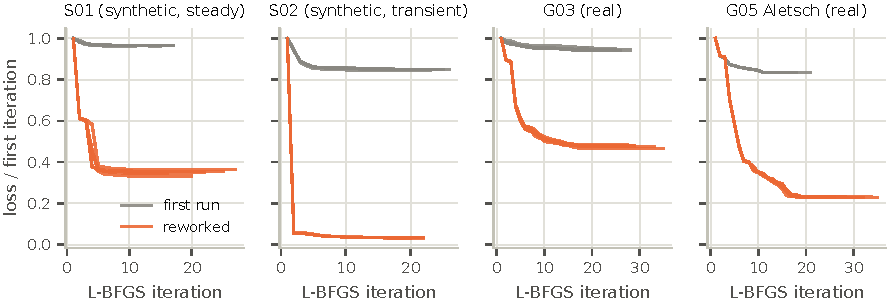
\includegraphics[width=\textwidth]{fig_loss_examples.pdf}
\caption{Loss of every family member, relative to its first iteration. The old loss flattens at 83--97\,\% of its start; the reworked loss keeps decreasing.}
\end{figure}

\begin{figure}[H]
\centering
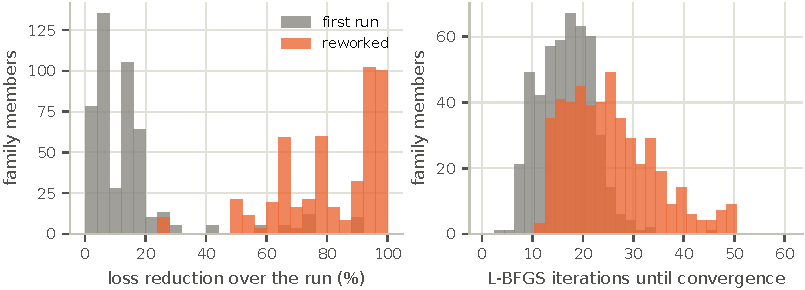
\includegraphics[width=0.78\textwidth]{fig_loss_all.pdf}
\caption{All \nMemNew\ family members. Median loss reduction \redMedOld\,\% $\to$ \redMedNew\,\%; \redBelowFiveOld\,\% of the old runs reduced the loss by less than 5\,\%, none of the new ones.
Median iterations \itsMedOld\ $\to$ \itsMedNew. The two losses are not the same quantity (cell RMSE vs.\ band misfit plus geodetic term), so Fig.~\ref{fig:thk} gives a common yardstick.}
\end{figure}

\begin{figure}[H]
\centering
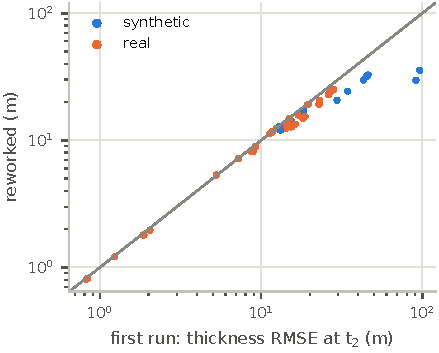
\includegraphics[width=0.42\textwidth]{fig_thk_rmse.pdf}
\caption{\label{fig:thk}Per-cell thickness error at $t_2$ (not what the new loss optimises) for the \thkN\ pairs: lower in \thkBetter; median \thkMedOld\,m $\to$ \thkMedNew\,m.}
\end{figure}

\section*{Results}
\begin{figure}[H]
\centering
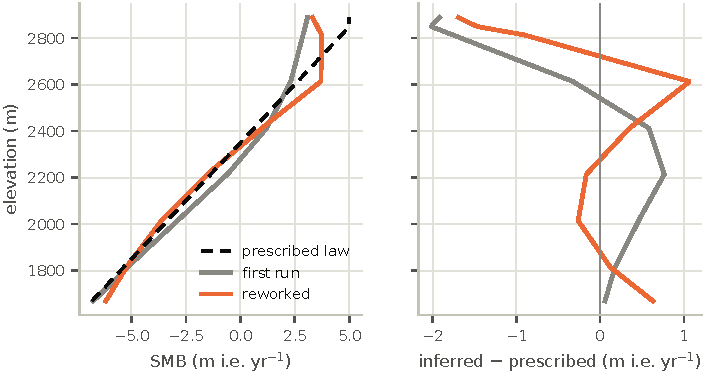
\includegraphics[width=0.78\textwidth]{fig_s01_profile.pdf}
\caption{S01 (EXP01), family-mean SMB profile against the prescribed law (RMSE \sOneOld\,$\to$\,\sOneNew\,\mie).}
\end{figure}

\begin{figure}[H]
\centering
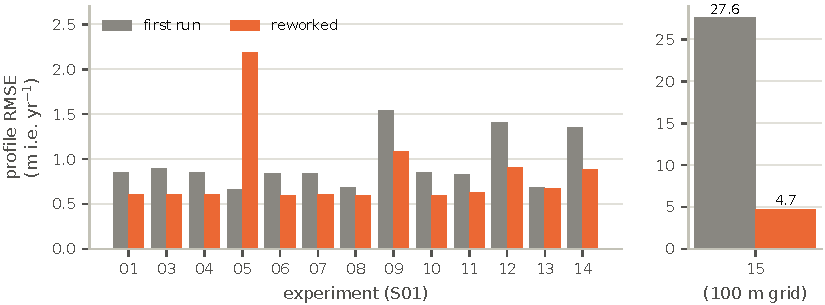
\includegraphics[width=\textwidth]{fig_s01_all.pdf}
\caption{All S01 experiments: profile RMSE against the prescribed law. Better in \sOneBetter\ of \sOneN; worse in \sOneWorse. In EXP05 the thickness
perturbation puts ice below the real terminus, so the ice mask reaches 230\,m lower and the glacier-wide constraint follows that inconsistent data.}
\end{figure}

\begin{figure}[H]
\centering
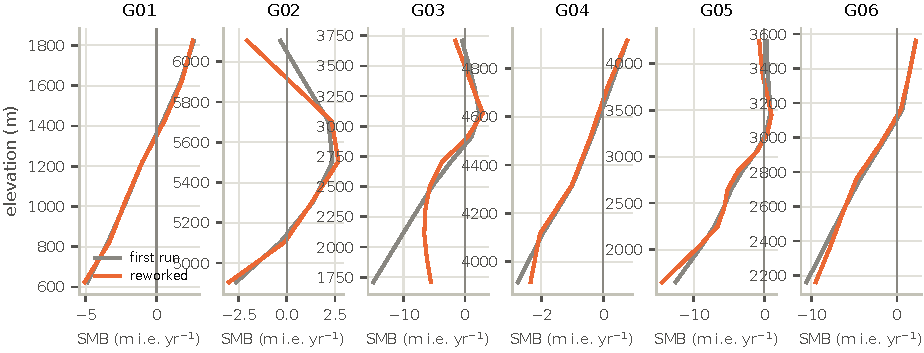
\includegraphics[width=\textwidth]{fig_real_profiles.pdf}
\caption{Real glaciers (EXP01), family-mean SMB profiles. Most are close to the first run; G03 changes most (its terminus touches the domain edge, where the old
ramp removed ice).}
\end{figure}

\begin{figure}[H]
\centering
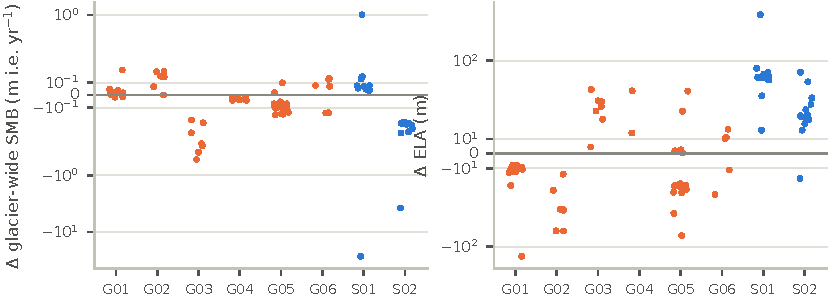
\includegraphics[width=\textwidth]{fig_shift.pdf}
\caption{Change (reworked minus first run) of glacier-wide SMB and ELA, one dot per experiment (symmetric-log axes). Median $|\Delta$SMB$|$ \gwShiftMed\,\mie\
(real glaciers \realGwShiftMed); median $|\Delta$ELA$|$ \elaShiftMed\,m. The large S01 changes are EXP15, whose coarse grid had failed in the first run
(glacier-wide SMB error $+27$\,\mie). Median $\sigma_\mathrm{SMB}$: \uncOld\ $\to$ \uncNew\,\mie.}
\end{figure}

\section*{Remaining limits}
\begin{itemize}\setlength\itemsep{0pt}
\item S01 is not fitted exactly. With model-generated data the inversion recovers the law (RMSE 0.05); with the observed data the error comes from the DA state
(ice volume 1.7--1.9$\times$ the truth, speed too low), not from the optimiser, regularisation or profile resolution.
\item The fixed step is chosen from the initial speeds. In one member (EXP20 G01, $\tau_\mathrm{ref}=1.79$) the run diverged; it was rerun with a halved CFL number (0.1).
\item The new results are in \texttt{results/<EXP>\_<GID>\_cnn/smb\_G\_bands\_geod/export/}; \texttt{GROUP\_UNIL/} still holds the first run.
\end{itemize}

\end{document}
